\section{The five-vertex path}\label{sec:five-chain}
Write the core in path order as
\[
 t\;--_{L_-}\;r\;--_{M_-}\;c\;--_{M_+}\;w\;--_{L_+}\;z,
 \qquad L_-,M_-,M_+,L_+\ge1.
\]
Here $L_\pm$ counts a terminal connector and $M_\pm$ the connector
from an off-center root to $c$. In a local outlet formula, $L$ denotes
the terminal-connector length and $M$ the receiving-connector length.
After Lemma~\ref{lem:five-reduction}, the two terminal residuals have
at least two entries and the three internal residuals are nonempty.
Call an internal residual S if it is a singleton and R otherwise.

\subsection{A central singleton: the maximal S spine}
Suppose $c$ is S. Take the maximal consecutive S sequence among
$r,c,w$ that contains $c$. Orient its singleton arms alternately as
$f_a$ and $\bar f_b$, starting with an outward arm at its left end.
Every connector between consecutive S vertices points from the
negative end toward the positive end. The corresponding operators
between square roots of the actual arm messages are
\[
 B_i=\sqrt{f_a}T^{M_i}\sqrt{\bar f_b}
 \quad\hbox{or their adjoints},\qquad \|B_i\|\le1
\]
by Proposition~\ref{q3:prop:operators}.

At a positive S end whose arm has message \(f_s\), an ordinary
terminal supplies
\[
 y=\sqrt{f_s}\,T^LF_t,\qquad \|y\|_2\le1,
\]
where \(F_t\) is positive canonical for an even residual list and
negative canonical for an odd residual list; the norm bound is
\eqref{q3:eq:singleendpoint}. An R half-tree supplies instead
\[
 y=\sqrt{f_s}\,T^MH,\qquad
 H=C^-TG=\sqrt q\,h,\qquad \|h\|_2\le1.
\]
Equations~\eqref{eq:inverse-half} and~\eqref{eq:five-normalized}
give \(\|y\|_2\le1\) for every \(M\ge1\).
At a negative S end reverse the entire outside configuration:
the two endpoint functions become
\(\sqrt{\bar f_s}A^LF_t^-\) and
\(\sqrt{\bar f_s}A^MH^-\), respectively, with the same norm bound.

Bounding the genuine equal-pair factors on the spine by one gives
\[
 \ip{y_L}{B_1\cdots B_{j-1}y_R}\le1,
 \qquad \|y_L\|_2,\|y_R\|_2\le1.
\]
For a one-vertex spine this is $\ip{y_L}{y_R}$. This covers the patterns SSS, RSS,
SSR and RSR. The two square roots of each arm contribute one arm factor, and each
original connector appears once.

\subsection{A unit off-center arm with a unit receiving connector}
Now suppose the center is R and, say, $r$ has one unit residual arm
and its receiving connector $r-c$ has $M_-=1$. Put $L=L_-$ and choose the terminal direction with
step count $L-1$. Its composite message at $r$ is
\[
 F_*^+=E_r^-qA^LF^-_{t,L-1}.
\]
The actual unit arm is the factor $q$. Row H\"older and $pq\le1$ give,
for every real $G$,
\[
 \E[q|pTG|^4]\le\E[(pq)^4T(|G|^4)]\le\E[p|G|^4].
\]
Full reversal proves $\E[p(F_*^+)^4]\le1$. The one edge from $r$ to
$c$ has not yet been integrated. Choose the central negative R factor
$C^-$ with $\E[q(C^-)^4]\le1$ and put $H_c=C^-TF_*^+$.
Lemma~\ref{lem:halftree} gives $N_+(H_c)\le1$.

At $w$, use the right R or S construction in Table~\ref{tab:roles},
with its actual terminal and terminal-connector length $L_+$. It gives a message
$H_w$ with $N_-(H_w)\le1$. Direct the entire $M_+$-path from $c$ to
$w$. The exact density is
\[
 Z_D=\ip{H_c}{A^{M_+}H_w}\le1.
\]
This whole-tree construction replaces the $I_q$ outlet at $r$.

\subsection{Two compatible outlets}
In the remaining structural branch $c$ is R, and any unit singleton
off-center has receiving-connector length at least two. Choose the central negative
zero-step factor $C_c$ as follows. An even residual uses negative
canonical pairs. An odd residual beginning with one uses
$E_c^-p\bar f_aW_b$ followed by negative canonical pairs. A nonunit
odd residual uses $E_c^+f_a$ followed by positive canonical pairs.
These are the full reversals of the corresponding zero-step
directions, so
\[
 \E[qC_c^4]\le1.
\]
Proposition~\ref{prop:five-outlet} supplies actual outputs $U_-,U_+$
for the two sides, both using this same $q$. Integration over their
disjoint interiors gives $Z_D=\E[C_cU_-U_+]$.
H\"older at exponents $4,8/3,8/3$ yields
\begin{align}\label{eq:five-chain-close}
 Z_D&\le(\E[qC_c^4])^{1/4}
             I_q(U_-)^{3/8}I_q(U_+)^{3/8}\notag\\
 &\le e^{-(\eta_-+\eta_+)d/8}\le e^{-d/2000}\le1.
\end{align}
The weight powers $1/4,-1/8,-1/8$ cancel, and both side functions are evaluated at the same central label.

\begin{figure}[htbp]\centering
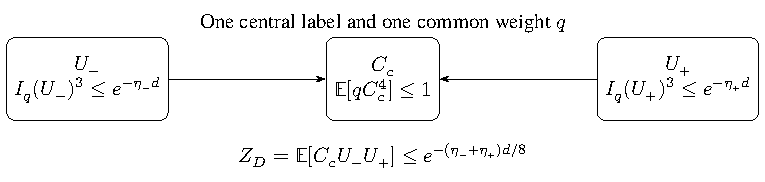
\includegraphics{figures/five-path-closure.pdf}
\caption{The remaining path branch. The two structural alternatives are applied first; only then are the two local outlets joined with the same central reference weight.}\label{fig:five-path}
\end{figure}

The root catalogue divides nonempty residual lists into singletons,
pairs, odd lists of at least three entries, and even lists of at least four. Singletons split according to their arm and
receiving-connector lengths: the two-step construction treats an arm of
length two differently from one of length at least three, and the choice
depends on the length; $d$ enters in the estimates. The minimum-two odd row with a
terminal $(2,t)$ has its own first-edge choices, notably $W_2\bar f_t$ at
$L=1$ and $\bar f_2W_t$ at $L\ge2$; the table in the technical appendix
lists them all. Together with the two whole-tree alternatives above,
\eqref{eq:five-chain-close} proves every $P_5$.

\subsection{A worked five-branch example}\label{sec:five-example}
Consider the path core in Figure~\ref{fig:five-example}, with connector
lengths \((L_-,M_-,M_+,L_+)=(2,1,2,1)\) and pendant-arm lists
\begin{equation}\label{eq:five-example:arms}
\begin{array}{c|ccccc}
 \text{vertex}&t&r&c&w&z\\\hline
 \text{arm lengths}&(2,4)&(1,3,4)&(4,5)&(2,4,5)&(2,3).
\end{array}
\end{equation}
This tree has 45 edges and five branch vertices, of degrees
\(3,5,4,5,3\). It falls in the two-outlet case above.
Direct every core edge toward \(c\), and choose the pendant directions
specified by the following messages:
\begin{equation}\label{eq:five-example:messages}
\begin{aligned}
 F_-&=\bar f_2W_4,& H_-&=pW_3\bar f_4\,T^2F_-,&U_-&=TH_-,\\
 F_+&=W_2\bar f_3,& H_+&=f_2h_4f_5\,TF_+,&U_+&=T^2H_+,\\
 &&C&=W_4\bar f_5.
\end{aligned}
\end{equation}
Integration over the two sides gives \(Z_D=\E[CU_-U_+]\).
We verify the three moment inputs to this identity directly.
When \(d=0\), leaf integration gives \(Z_D=1\); henceforth assume \(d>0\).

\begin{figure}[htbp]\centering
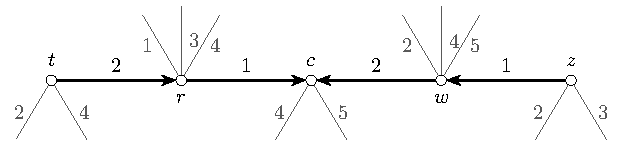
\includegraphics{figures/five-branch-example.pdf}
\caption{The five-branch example. Each segment represents a path of
the indicated length; pendant directions are specified in
\eqref{eq:five-example:messages}.}\label{fig:five-example}
\end{figure}

Put \(B=-K\) and \(u=-g=B\one\), so that \(T=J+B\),
\(A=J-B\), \(p=1-u\), and \(q=1+u\). We use
\(d\le1/3\), \(\delta_{j+1}\le\theta\delta_j\),
\(\theta=13/32\), and the spectral measure \(\nu\) of \(-B^2\)
at \(u\), for which \(\int x^j\,d\nu=\delta_{j+1}\).
The row bound \(|BV|\le\|V\|_2\) and
\eqref{eq:oc:signed-moments} give the common fourth-moment rule
\begin{equation}\label{eq:five-example:payment}
 0\le H\le e^{a+BV}\quad\Longrightarrow\quad
 \log\E H^4\le4(a+\E BV)+\tfrac{17}{4}\|V\|_2^2.
\end{equation}
The arm recurrences \(f_{n+1}=Af_n\),
\(\bar f_{n+1}=T\bar f_n\), \(h_n=Tf_{n-1}\), and
\(W_n=A\bar f_{n-1}\) give
\begin{equation}\label{eq:five-example:identities}
\begin{aligned}
 \bar f_2+W_4&=2-2d+du-B^2u-B^3u,\\
 W_3+\bar f_4&=2-3d-du+B^3u,\\
 W_2+\bar f_3&=2-d+B^2u,\\
 h_4+f_5&=2-4d+\delta_2-df_2-B^4u,\\
 W_4+\bar f_5&=2-4d+\delta_2-d\bar f_2+B^4u.
\end{aligned}
\end{equation}
These identities and \(ab\le e^{a+b-2}\) for nonnegative \(a,b\)
provide all the envelopes below.

\paragraph{The two-step side.}
Set
\[
 R=du-B^2u-B^3u,\quad s=\E R^2
   =d^3+2d\delta_2+\delta_3+\delta_4,\quad
 \Delta=-\delta_2+\tfrac32s,
 \quad\epsilon=\Delta-d^2-\delta_2.
\]
The first identity gives \(F_-\le e^{-2d+R}\).
Since \(|R|\le d+\sqrt{\delta_2+\delta_3}<1\), the elementary
bound \(e^y\le1+y+3y^2/4\), \(|y|\le1\), and positivity give
\[
 TF_-\le e^{-2d}(q+BR+\Delta),\qquad
 T^2F_-\le e^{-2d}(\bar f_2+B^2R+\Delta q-d^2-\delta_2).
\]
Adding the factors in the last upper bound to \(p\), and then using
the second identity in \eqref{eq:five-example:identities}, yields
\[
 H_-\le e^{-5d+\epsilon+BV_-},\qquad
 V_-=u+BR+B^2u+(\Delta-d)\one.
\]
Here
\[
 -5d+\epsilon+\E BV_-
 =-6d+\epsilon+\delta_2+\delta_3<-\tfrac{27}{5}d.
\]
Indeed
\[
 \epsilon=d^2(-1+3d/2)+(-2+3d)\delta_2
                     +\tfrac32(\delta_3+\delta_4)\le0,
\]
because \(3\theta(1+\theta)/2<1\).

To bound the complete vector, write \(c_0=\Delta-d\). Its
nonconstant part has spectral coordinates
\(a(x)=1-x-x^2\), \(b(x)=d+x\).
On \([0,\theta]\), \(a^2\le1-x\) and \(0\le b\le1\),
so that part has squared norm at most \(d\) and mean
\(-d^2-\delta_2\). Moreover
\[
 s/d\le\tfrac19+\tfrac{2\theta}{3}+\theta^2+\theta^3<\tfrac58,
 \qquad -(d+\delta_2)\le c_0<0.
\]
Keeping its constant cross term therefore gives
\[
 \|V_-\|_2^2\le d+(d+\delta_2)^2
                +2(d+\delta_2)(d^2+\delta_2)<\tfrac{12}{5}d.
\]
The rule \eqref{eq:five-example:payment} now proves
\(\log\E H_-^4<-57d/5\le-6d\).

\paragraph{The one-step side.}
The third identity gives
\(F_+\le e^{-d+B^2u}\). The same Taylor bound gives
\[
 TF_+\le e^{-d}(q+B^3u+\tfrac32\delta_3).
\]
Adding its upper factor to \(f_2=1-u+Bu\) leaves
\(2+B(u+B^2u)+3\delta_3/2\). The fourth identity, together
with \(f_2\ge0\) and \(4-\theta>3\), gives
\(h_4f_5\le e^{-3d-B^4u}\). Consequently
\[
 H_+\le e^{-4d+(3/2)\delta_3+BV_+},\qquad
 V_+=u+B^2u-B^3u.
\]
Its spectral square is \((1-x)^2+x^3\le1\). Thus
\[
 \|V_+\|_2^2\le d,\qquad
 -4d+\tfrac32\delta_3+\E BV_+
 =-5d+\delta_2+\tfrac32\delta_3<-4d.
\]
Equation~\eqref{eq:five-example:payment} proves
\(\log\E H_+^4<-47d/4\le-6d\).

\paragraph{The center and the receiving connectors.}
The last identity gives \(C\le e^{-3d+B^4u}\).
Put \(X=u+4B^4u\). Skew-adjointness gives \(\E X=0\), and
\[
 |X|\le1+4\theta^{3/2}\sqrt d<2,\qquad
 \E X^2\le(1+4\theta^2)^2d<3d.
\]
Since \(q\le e^u\) and \(e^y\le1+y+3y^2/2\) for \(|y|\le2\),
\[
 \E[qC^4]\le e^{-12d}\E e^X
 \le e^{-12d}(1+9d/2)\le e^{-15d/2}\le1.
\]
For a positive operator \(P\), row Cauchy--Schwarz followed by
H\"older gives
\[
 I_q(PH)^3\le\E[(P\one)^4/q]\,\|P\|_{2\to2}^4(\E H^4)^2.
\]
The short-path row and operator bounds proved in
Section~\ref{proof:Q5-C084} are
\[
 \E[q^3]\le e^{4d},\quad \|T\|^4\le e^{128d/19},\qquad
 \E[\bar f_2^4/q]\le e^{6d},\quad \|T^2\|^4\le e^{4d}.
\]
Using \(\E H_-^4,\E H_+^4\le e^{-6d}\) gives
\[
 I_q(U_-)^3\le e^{-24d/19},\qquad I_q(U_+)^3\le e^{-2d}.
\]
Finally, the three-factor H\"older inequality at \(c\) yields
\[
 Z_D\le(\E[qC^4])^{1/4}
           I_q(U_-)^{3/8}I_q(U_+)^{3/8}
 \le e^{-(24/19+2)d/8}\le1.
\]
The powers \(q^{1/4},q^{-1/8},q^{-1/8}\) cancel at the central
label.

